\section{Schaltungsentwurf - Sendeeinheit}
\subsection{Spannungsversorgung}
\begin{floatingfigure}[r]{6.5cm}
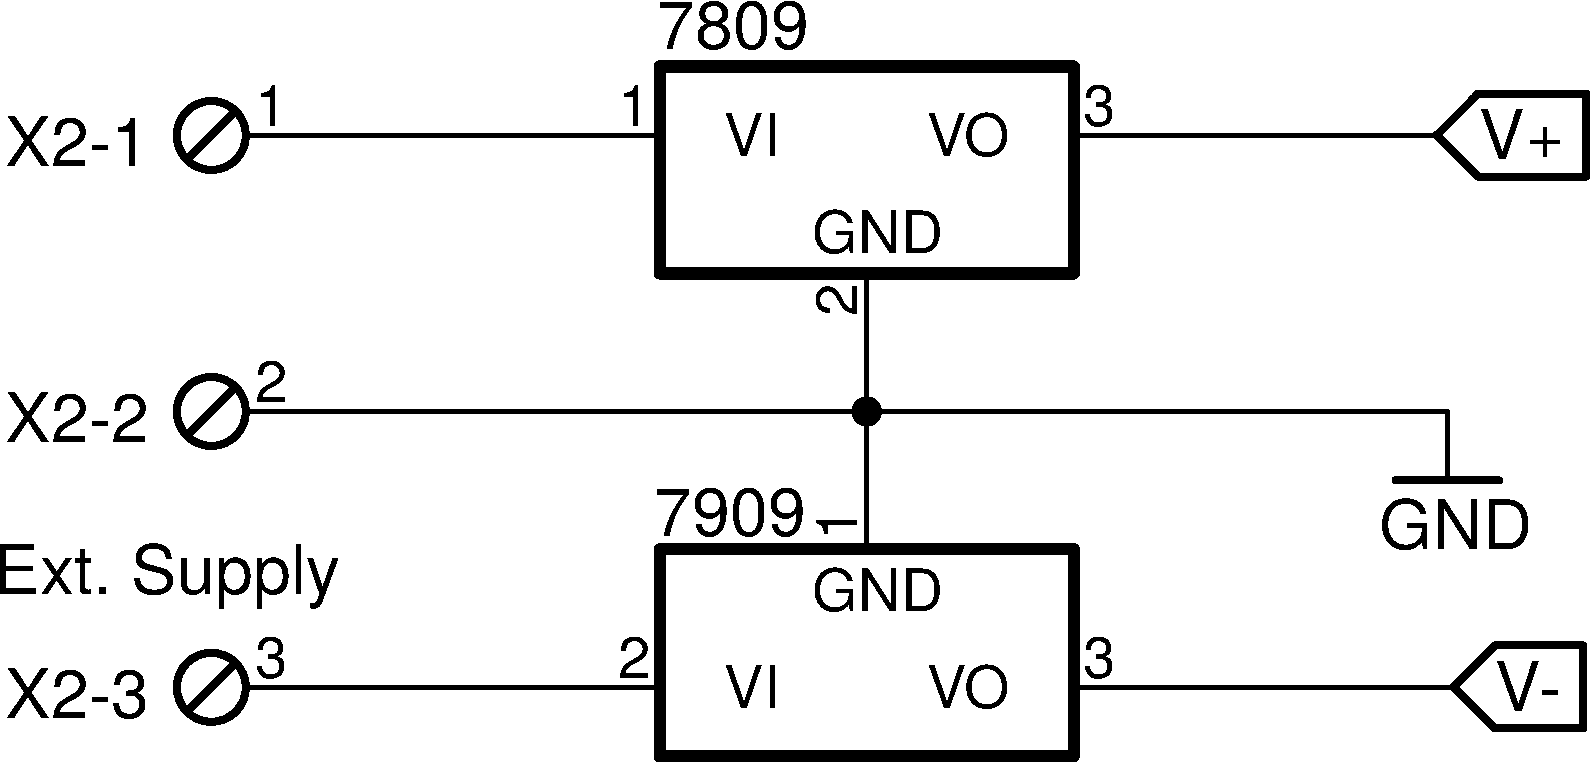
\includegraphics[width=6cm]{gfx/vcc.pdf}
\caption{Spannungsversorgung}
\label{fig:vcc}
\vspace{0.5cm}
\end{floatingfigure}
\noindent
Die Spannungsversorgung für die Sendeeinheit erfolgt zur galvanischen Trennung über Batterien. Aufgrund der hohen Stromaufnahme durch die Sendediode sowie der Status-LEDs ist eine interne Versorgung über 9V Blockbatterien nur bedingt möglich. Deswegen wird auf eine externe Versorgng über 12V Akkus zurückgegriffen. Damit die Schaltung dennoch bei allen Akkuspannungen zuverlässig und mit gleichen Ergebnissen arbeitet wird die Spannung intern auf 9V stabilisiert.